\documentclass[letterpaper,12pt]{article}

\usepackage{rotating}
\usepackage[top=1in, bottom=1in, left=1in, right=1in]{geometry}
\usepackage{graphicx}
\usepackage[numbers,square,sort&compress]{natbib}
\usepackage{setspace}
\usepackage[cdot,mediumqspace,]{SIunits}
\usepackage{hyperref}
\usepackage{mathtools}

\usepackage{amsmath}
\begin{document}
\onehalfspacing
\title{Photon Counting and Statistics of Light}
\author{Anita Bahmanyar, Ayushi Singh, Carly Berard}
\date{30 September, 2013}

%Title
\maketitle
\begin{abstract}
\label{abstract}
Randomness is a phenomena that occurs often in the nature. Counting the number of photons would be one example of it.  
\end{abstract}

%Introduction
\section{Introduction}
\label{sec:introduction}
In this experiment, we will use the light detector device called Photomultiplier Tube, also known as PMT, in order to count the number of light particles(photons). The photometer consisted of PMT photon counting Head H10682, a counter and a computer which the PMT was connected to. The goal of this experiment is to show the randomness of the photons hitting the device and to show what the role of statistical methods in counting the photons is. Python programming language will be used to plot data and analyze them. Another aim of this lab would be to see what the limitations of detecting light is in astronomy.

%Experimental Procedure
\section{Experimental Procedure}
\label{sec:experimental procedure}
In order to take data, we first turned on PMT and ran its software on the main computer. Then, we used pmt.py python code to collect data. Afterwards, we wrote a small python code to  specify the sampling time and number of counts per second and finally we plotted the data, both normally and in histogram style. Figure 1 shows the number of counts of the photons and figure 2 shows the histograms of the same data(a more professional way of showing data, since it includes time as well) These plots show the randomness of photon count, since none of the plots are the same. In order to get the count rate, one should divide the counts per sample by the sample time. For instance, here we could divide 100 by 0.001 to get the sample rate of 10000.

%Figure 1, photon counts normal plot
\begin{figure}
\centering
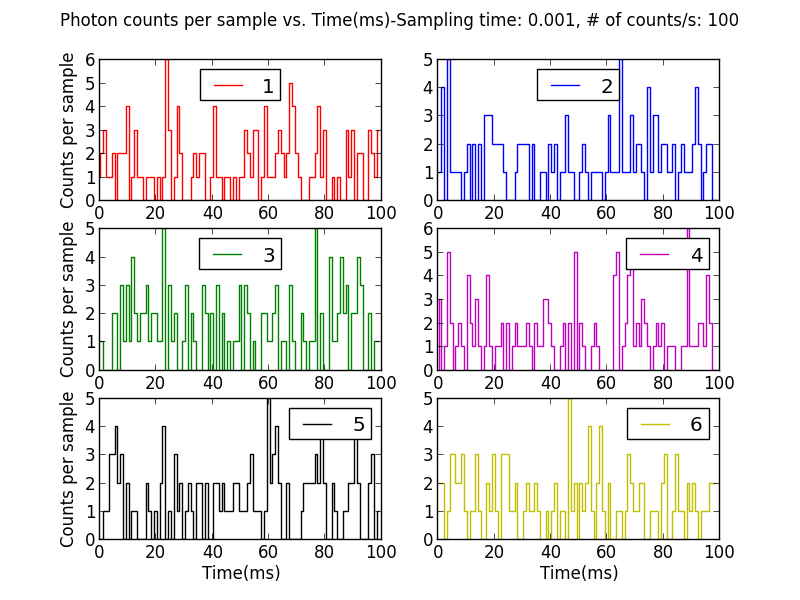
\includegraphics[scale=0.7]{ex_1_plot_1.png}
\caption{ Photon Count per Sample vs. Time plots}
The plots of number of counts versus time for sampling time of 0.001 and 100 photons per second. Six sets of data were taken with the same sampling time and count rate in order to show the randomness of the photon encounters. None of the plots are exactly the same; however, they have a similar overall shape.
\end{figure}

%Figure 2, histograms of photon counts
\begin{figure}
\centering
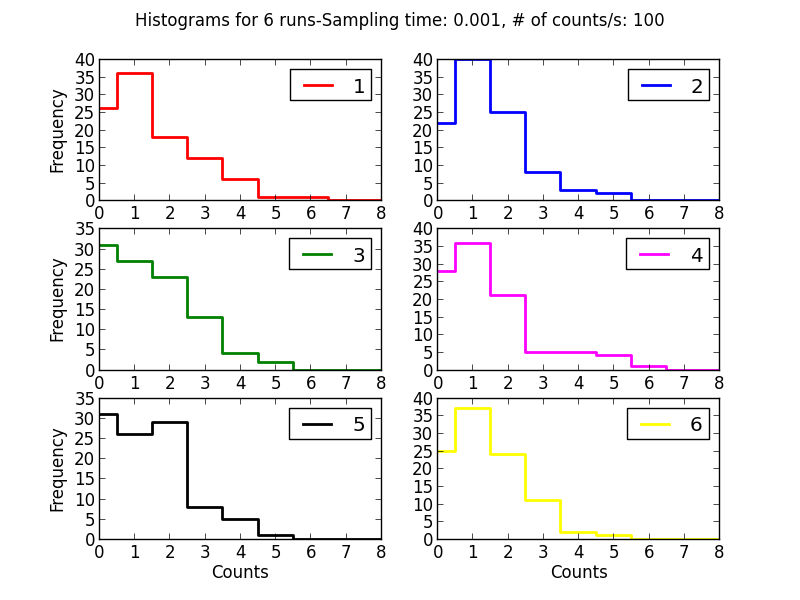
\includegraphics[scale=0.7]{histograms.png}
\caption{Histograms of Photon Counts}
The conclusion about this figure wold be the same as conclusion of figure 1.  The histograms provide a better way of showing data as it is much easier to read and interpret the data.
\end{figure}


As we progressed, we wrote python codes to make life much easier for collecting data. What this code did was that it ran a loop that collected data and saved it under different names each time. Therefore, we ended up getting all the files organized fast. I should also mention that Carly Berard mostly did the collection of data part and I should also give credit to Ayushi for collecting dark counts and some other parts throughout the lab. 
Other than collecting data when the light is on, we managed to collect data when the light was off to see what the difference would be. Then we plotted the same histogram plots for the dark count and the result is shown in figure 3. By looking at the picture we conclude that even when the light was off, the photomultiplier tube counted some photons and the reasons are explained in figure 3 caption.

%Figure 3, histograms of dark counts
\begin{figure}
\centering
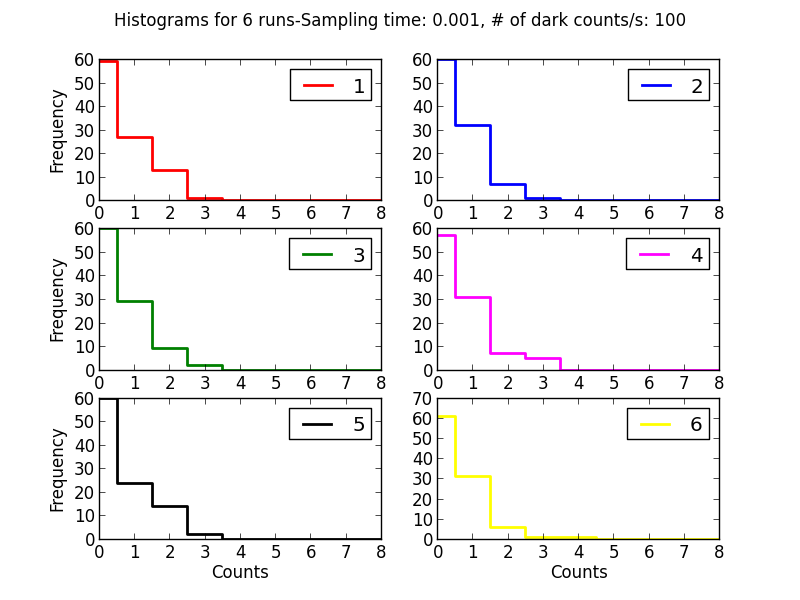
\includegraphics[scale=0.7]{Darkcounts1.png}
\caption{Histograms of dark counts}
This figure shows that even when the light is off, we will get some photons coming in. There might be a few reasonings behind it. First of all, even when the light was off, there was light in the room(it was not complete darkness). Secondly, the photons might also come from the error in the machine which might not be completely enclosed in darkness. Moreover, it could be due to the internal heat that would be releasing electrons.
\end{figure}

%Analysis
\section{Analysis}
\label{sec:analysis}
The next step would be to do some statistical analysis and to calculate the mean and the standard deviation of the data set. Therefore, we would know what the average value of our photon counts would be and we would also figure out how precise our measurements were.
The mean formula is given by equation 1, where n is the number of counts in total.
\begin{equation} \label{E:mean}
\bar{x} = \frac{\sum_{i=1}^{n}x_{i}} {n}
\end{equation}


And the standard deviation formula is given by equation 2:, where xi   (????) is each photon count and x bar (?????)is the mean value calculated by equation 1. 
%Mean equation
\begin{equation} \label{E:sd}
\sigma = \sqrt{\frac{\sum\limits_{i=1}^{n}
\left(x_{i} - \bar{x}\right)^{2}}
{n-1}}
\end{equation}

The smaller the value of the standard deviation, the more precise our measurements are. Table 1 shows the values of mean and standard deviation for data sets with similar sample rate and counts, repeated 6 times. Variance is the standard deviation squared. The plot of Variance vs. Number of Counts for Table 1 data set is shown in figure 4.

%Table 1
\begin{table}[ht]
\caption{Mean and Standard Deviation for 6 data sets with similar sample rate and time} % title of Table
\centering % used for centering table
\begin{tabular}{c c c c c} % centered columns (4 columns)
\hline\hline %inserts double horizontal lines
Data Set \# & Sample Rate & Counts(per s) & Mean of Counts & Standard Deviation \\ [0.5ex] % inserts table
%heading
\hline % inserts single horizontal line
1 & 1000 & 400 & 16.507 & 4.14\\ % inserting body of the table
2 & 1000 & 400& 16.69  & 3.93\\
3 & 1000 & 400& 16.405  & 4.08\\
4 & 1000 & 400 & 16.622 & 4.17\\
5 & 1000 & 400 & 16.922 & 4.10\\ 
6 & 1000 & 400 & 16.732 & 4.21 \\ [1ex] % [1ex] adds vertical space
\hline %inserts single line
\end{tabular}
\label{table:nonlin} % is used to refer this table in the text
\end{table}

%Figure 4, variance vs. count numbers for 400
\begin{figure}
\centering
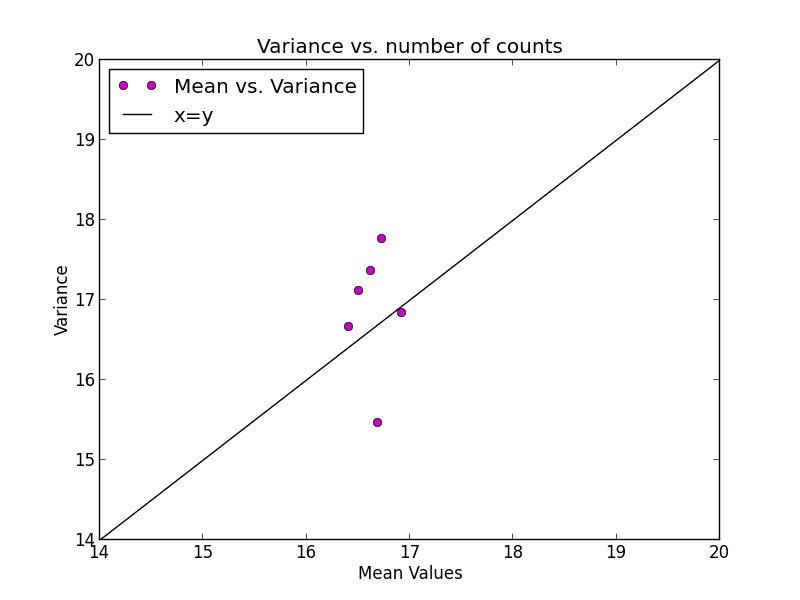
\includegraphics[scale=0.6]{variance-vs-count-number-400.png}
\caption{variance vs count number for table 1 data set}
\end{figure}

Figure 4 shows that the relation between variance and mean is almost linear.

%Figure 5, variance vs. count numbers all data set
\begin{figure}
\centering
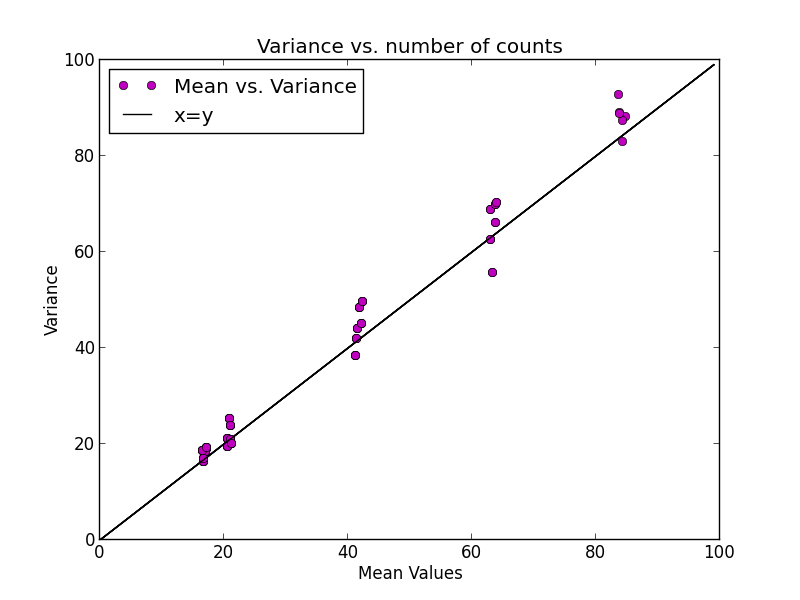
\includegraphics[scale=0.6]{variance-all-together.png}
\caption{variance vs count number for table 2 data set}
\end{figure}



%Table of mean vs. variance for 5 different data sets each with 6 data sets
\begin{table}[ht]
\caption{Mean and Standard Deviation for 5 data sets each consisting of 6 data sets} % title of Table
\centering % used for centering table
\begin{tabular}{c c c c c} % centered columns (4 columns)
\hline\hline %inserts double horizontal lines
Data Set \# & Sample Rate & Counts(per s) & Mean of Counts & Standard Deviation \\ [0.5ex] % inserts table
%heading
\hline % inserts single horizontal line
1 & 100 & 400 & 16.939 & 4.242\\ % inserting body of the table
2 & 80 & 400& 20.962  & 4.657 \\
3 & 40 & 400& 41.814 &  6.666 \\
4 & 26.67 & 400 & 63.558 & 8.085   \\
5 & 20 & 400 & 84.192 &  9.385 \\  [1ex] % [1ex] adds vertical space
\hline %inserts single line
\end{tabular}
\label{table:nonlin} % is used to refer this table in the text
\end{table}


%Table of dark counts and their mean values
\begin{table}[ht]
\caption{Mean and Standard Deviation for 4 dark data sets each consisting of 6 data sets } % title of Table
\centering % used for centering table
\begin{tabular}{c c c c c} % centered columns (4 columns)
\hline\hline %inserts double horizontal lines
Data Set \# & Sample Rate & Dark Counts(per s) & Mean of Dark Counts & Standard Deviation \\ [0.5ex] % inserts table
%heading
\hline % inserts single horizontal line
1 & 1000 & 1000 &  0.506 &  0.732   \\ % inserting body of the table
2 & 1000 & 100&   0.543   & 0.759 \\
3 & 100 & 100&    5.28  &  2.448      \\
4 & 100 & 400 &   5.153   &   2.326   \\  [1ex] % [1ex] adds vertical space
\hline %inserts single line
\end{tabular}
\label{table:nonlin} % is used to refer this table in the text
\end{table}


%Figure 6, Collage photo of mean vs. variance of dark counts
\begin{figure}
\centering
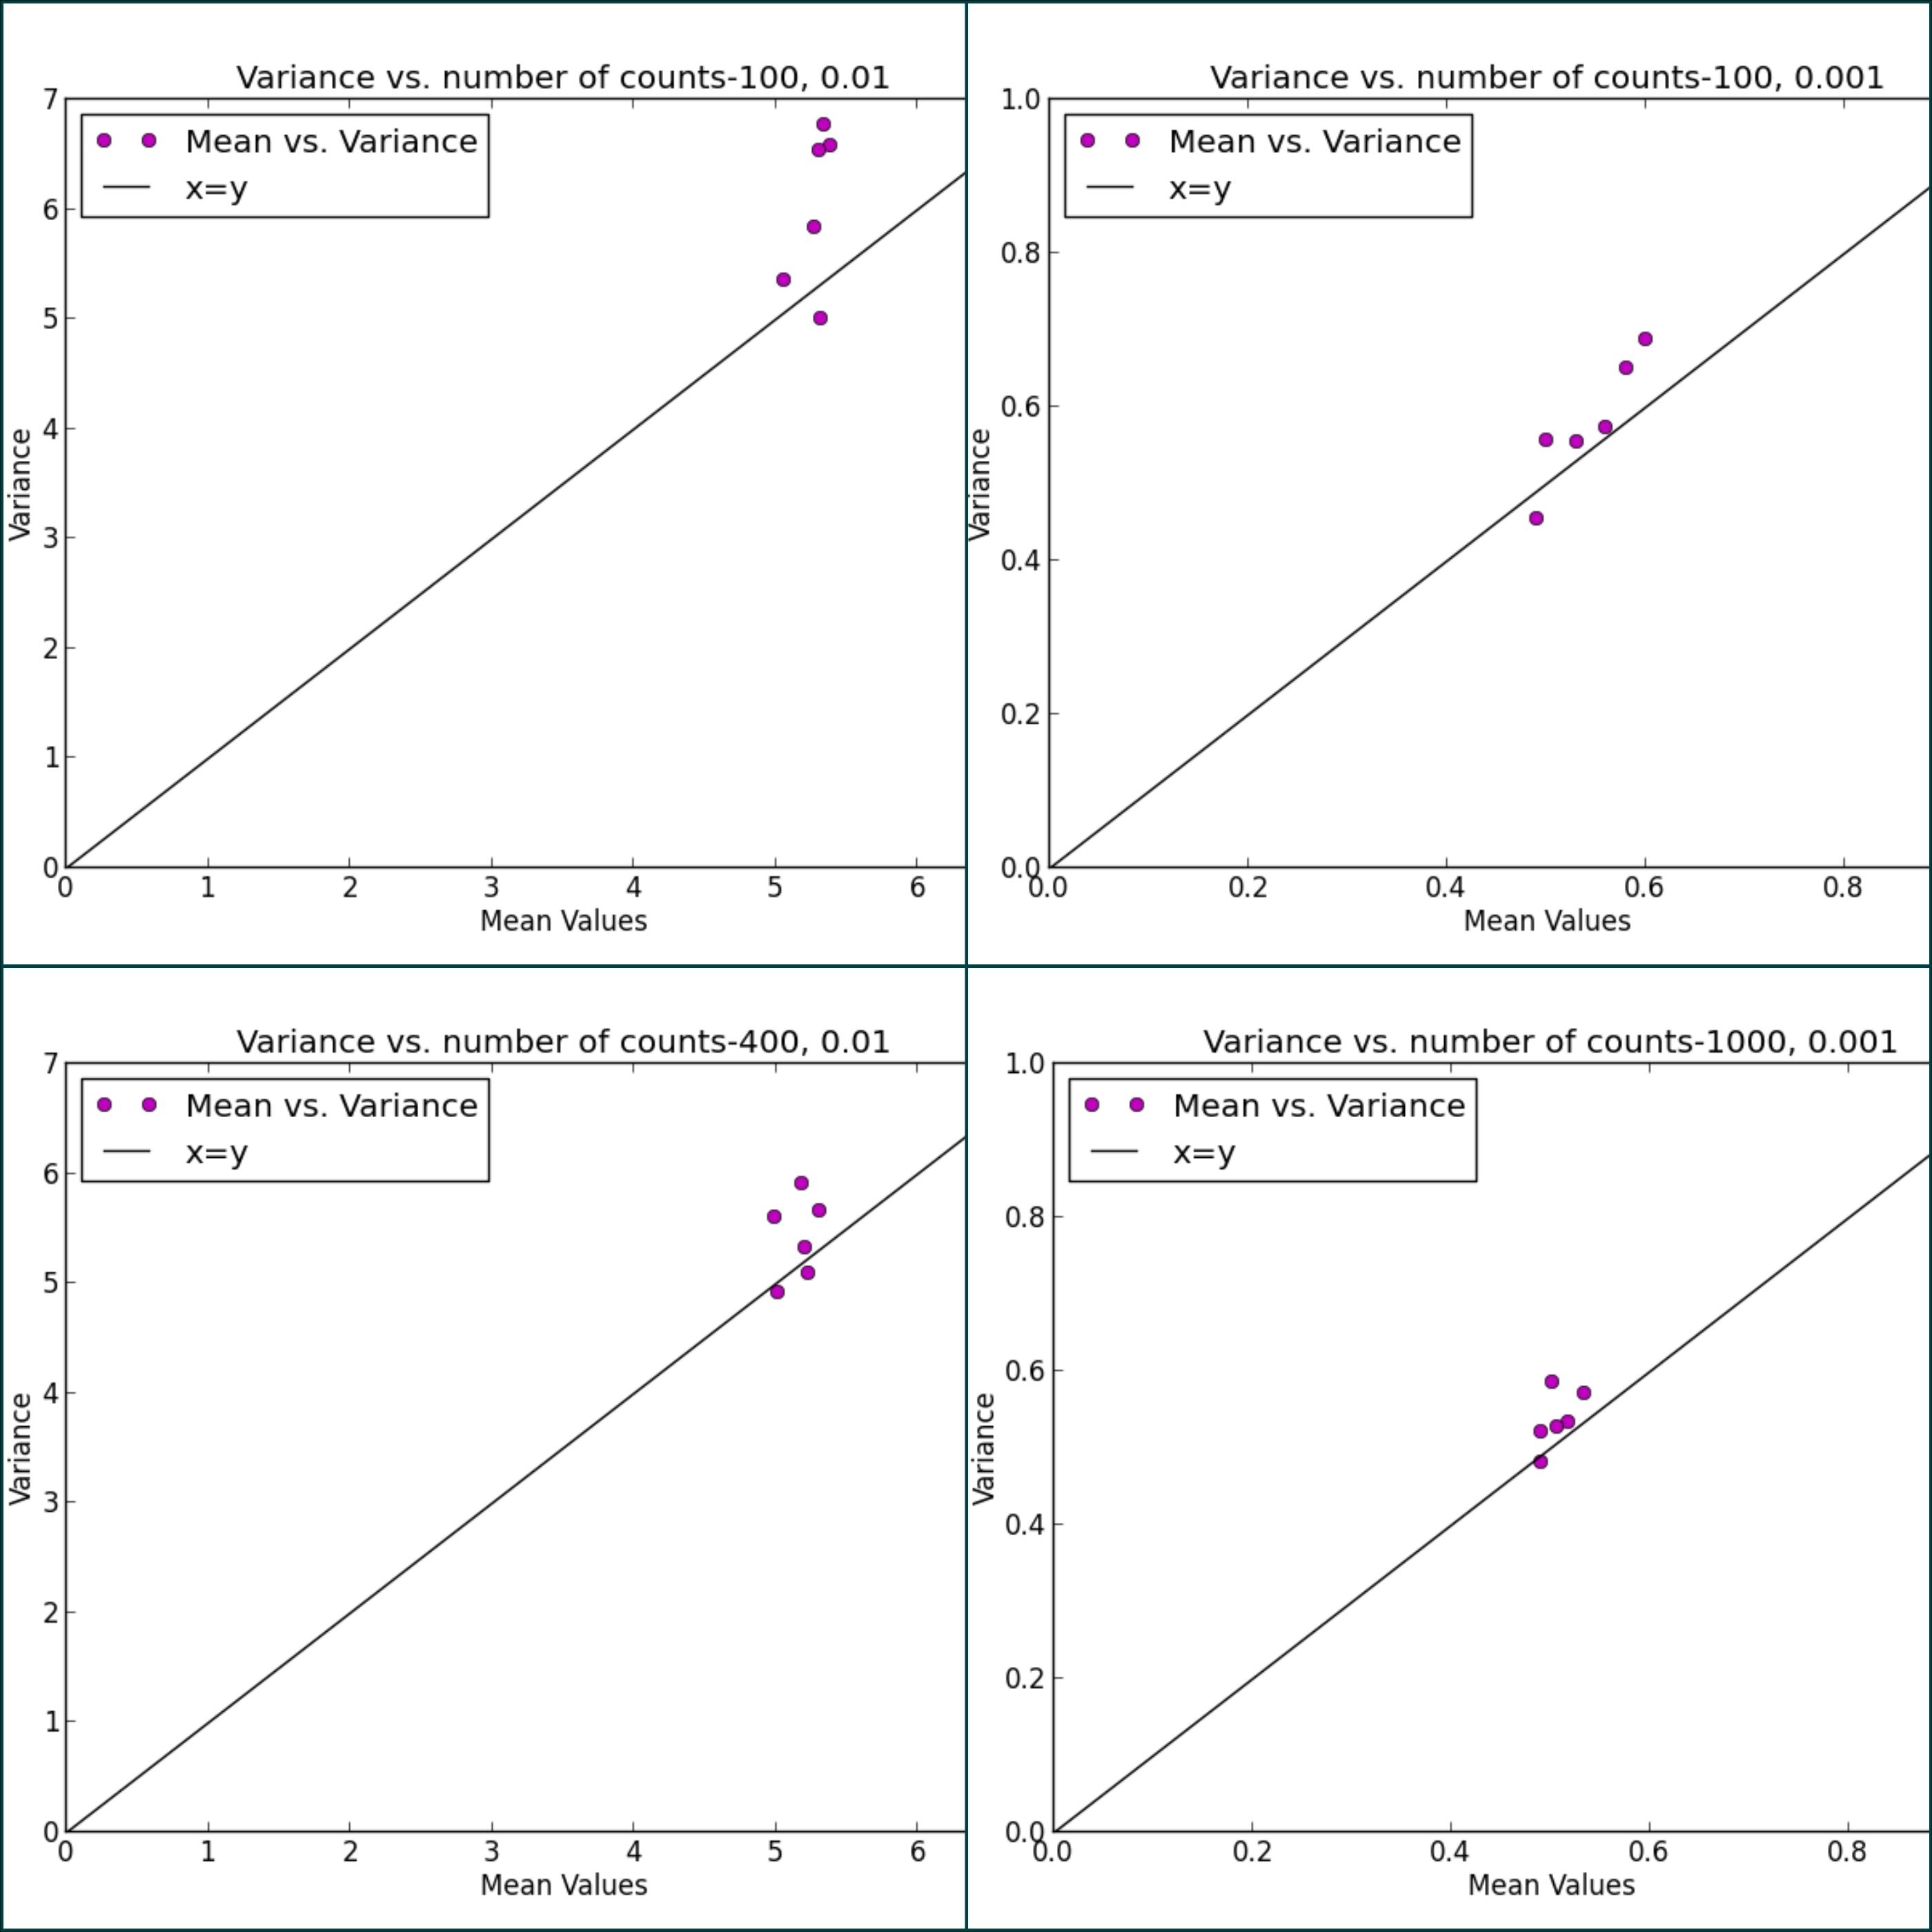
\includegraphics[scale=0.15]{dark_counts_400_0_Fotor_Collage.png}
\caption{variance vs dark count number for table 3 data set}
As it is visible in Table 3, as the sample rate and number of counts per second increase, the mean of the dark count and also the standard deviation decreases, meaning the data would be more precise as was also true for counts when the light was on.
\end{figure}

%Comparison with Theoretical Expectations
\section{Comparison with Theoretical Expectations}
\label{sec:comparison with theoretical expectations}
%poisson
\subsection{Poisson Distribution}
\label{sec:poisson distribution}
Poisson distribution predicts the probability of getting count rate for specific set of values which are descrete. Poisson distribution only depends on one variable, which is mean. It is independent of standard deviation and this is why it is easier to use rather than gaussian distribution. Poisson distribution is given by equation 3:

\begin{equation} \label{poisson} P\left( x \right) = \frac{{e^{ - \mu } \mu ^x }}{{x!}} \end{equation}
Where \begin{math}\mu \end{math} is the mean. 

%gaussian 
\subsection{Gaussian Distribution}
\label{sec:gaussian distribution}
Gaussian distribution is a continuous probability distribution. Gaussian is better for large count limit since the poisson distribution function becomes tedious to solve for large counts due to the factorial in the denominator. However, it is not good for small counts limit since we need two parameters to solve it: mean and standard deviation.
Gaussian distribution function is given by equation 4:

\begin{equation}
\label{gaussian}
P(x) = \frac{1}{{\sigma \sqrt {2\pi } }}e^{{{ - \left( {x - \mu } \right)^2 } \mathord{\left/ {\vphantom {{ - \left( {x - \mu } \right)^2 } {2\sigma ^2 }}} \right. \kern-\nulldelimiterspace} {2\sigma ^2 }}}
\end{equation}
Figure 7 shows the plots of poisson and gaussian distribution over the histogram plots of small values. It shows that poisson distribution is a better prediction than gaussian for small counts.

%figure 7, poisson-gaussian and histograms(part 8)
\begin{figure}
\centering
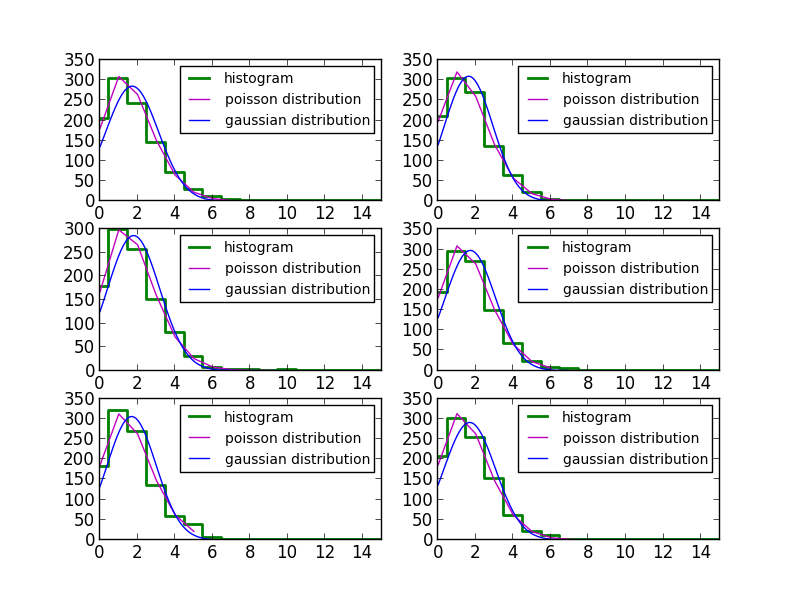
\includegraphics[scale=0.9]{poisson-gaussian-histograms-8.png}
\caption{Poissoon, Gaussian and Histograms of small count limit data sets}
Poisson distribution is a better approximation for small data sets as is shown in these plots.\end{figure}

 Also, poisson is a discrete distribution whereas gaussian is a continuous one. in the large count limit, the poisson distribution gets closer to gaussian distribution which is a good property; therefore, we would be able to solve gaussian function instead of poisson for large counts limit. In gaussian distribution, peak is at mean.
 
 %Figure 8, poisson-gaussian and histograms for large counts
 \begin{figure}
\centering
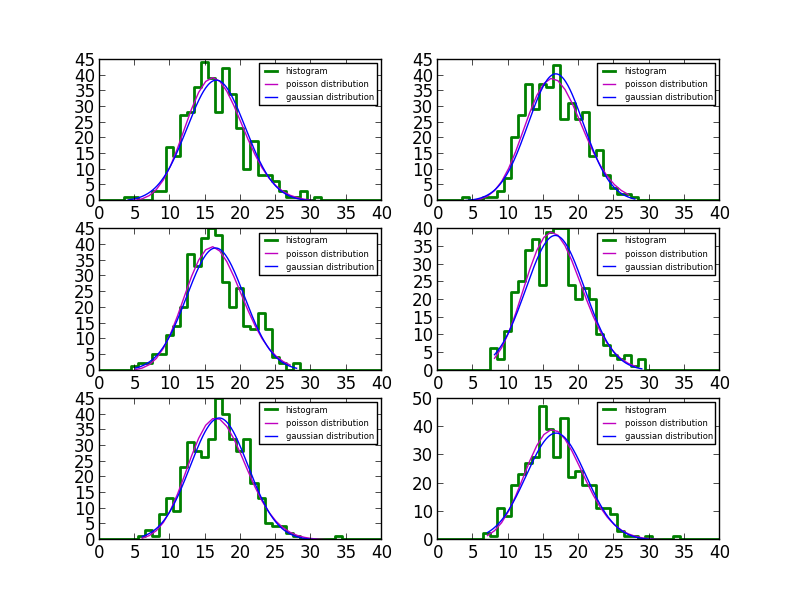
\includegraphics[scale=0.9]{poisson-gaussian-histograms-8-long.png}
\caption{Poissoon, Gaussian and Histograms of long count limit data sets}
Poisson and gaussian distribution are almost the same for long count limit as is seen in these plots. Therefore, it is more convenient to use gaussian distribution function for long limits rather than small count limit.
\end{figure}
 
 
 
 %Table 4, part 9, small to large counts and its effect on mean of mean and standard deviation of mean
 
 
 
 %Figure 9, MOM and SDOM, part 9 



\end{document}